\begin{figure}[p]
    \centering
    \begin{subfigure}{0.47\linewidth}
        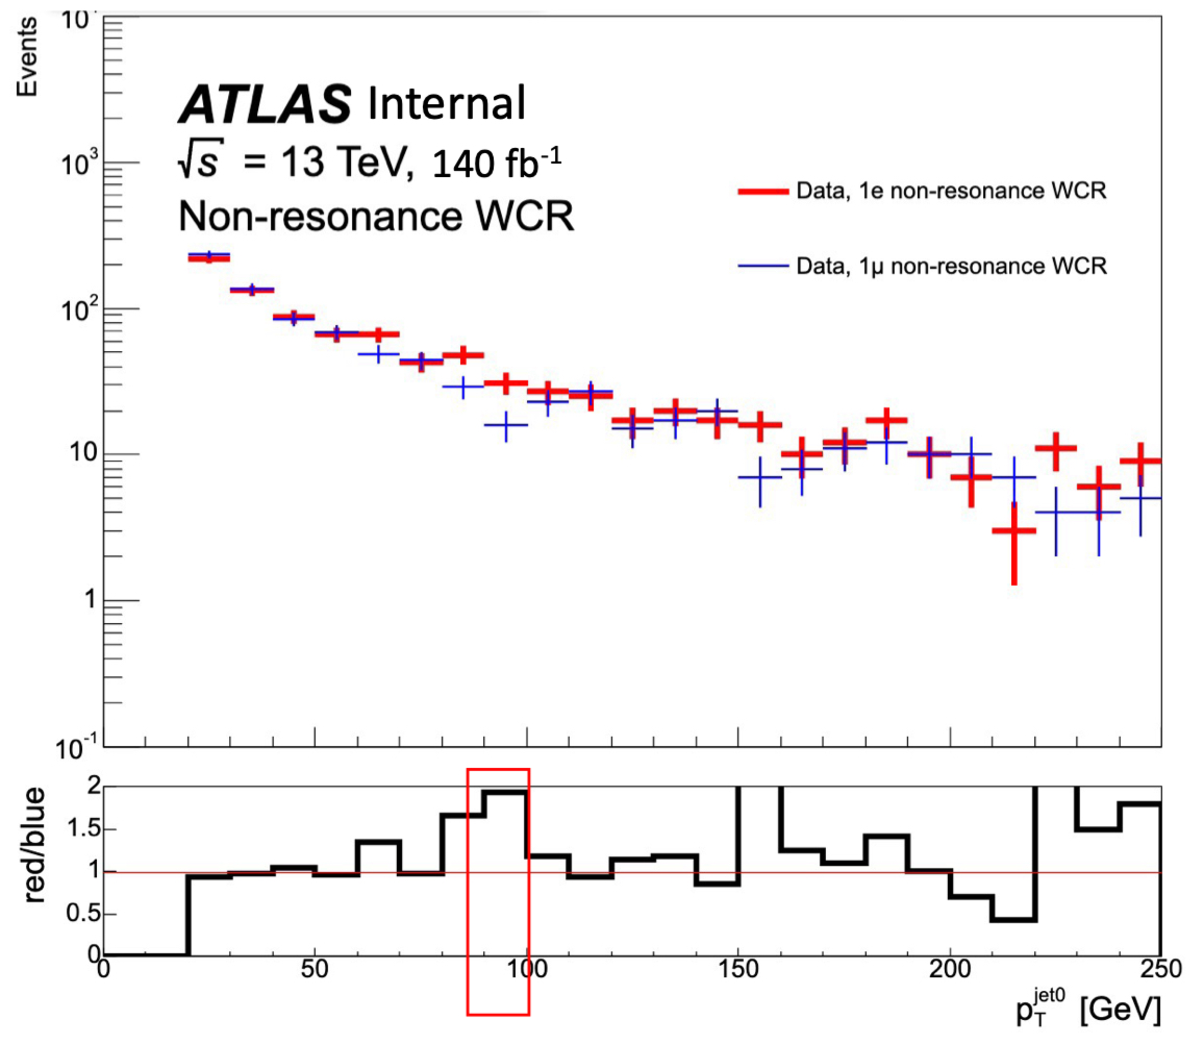
\includegraphics[width=\linewidth]{Figs/CH8/WCR_emuRatio_Data.pdf}
        \caption[]{Leading-jet $\pT$ in data}
    \end{subfigure}\hfill
    \begin{subfigure}{0.47\linewidth}
        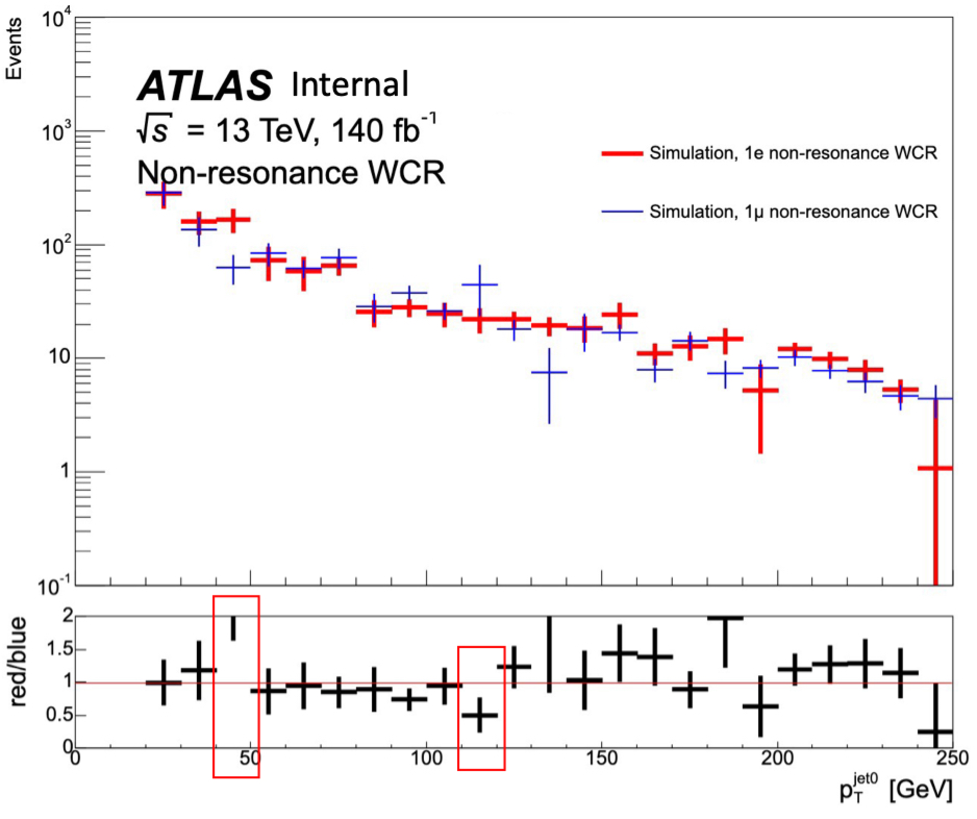
\includegraphics[width=\linewidth]{Figs/CH8/WCR_emuRatio_MC.pdf}
        \caption[]{Leading-jet $\pT$ in simulation}
    \end{subfigure}\par\medskip
    \begin{subfigure}{0.47\linewidth}
        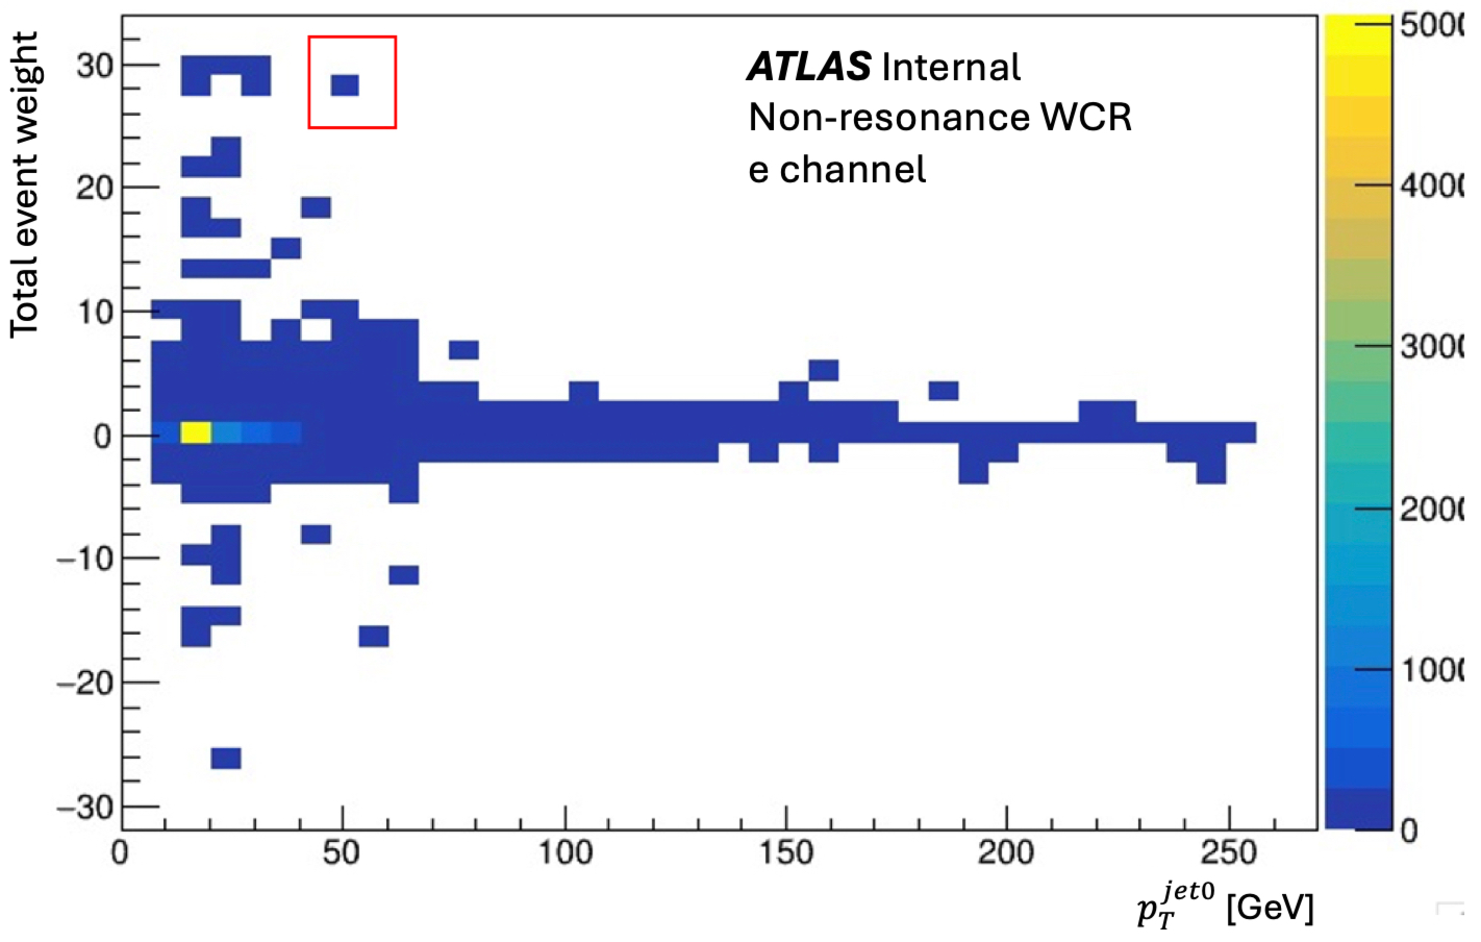
\includegraphics[width=\linewidth]{Figs/CH8/WCR_evenweight_e.pdf}
        \caption[]{Event weights in the electron simulation}
    \end{subfigure}\hfill
    \begin{subfigure}{0.47\linewidth}
        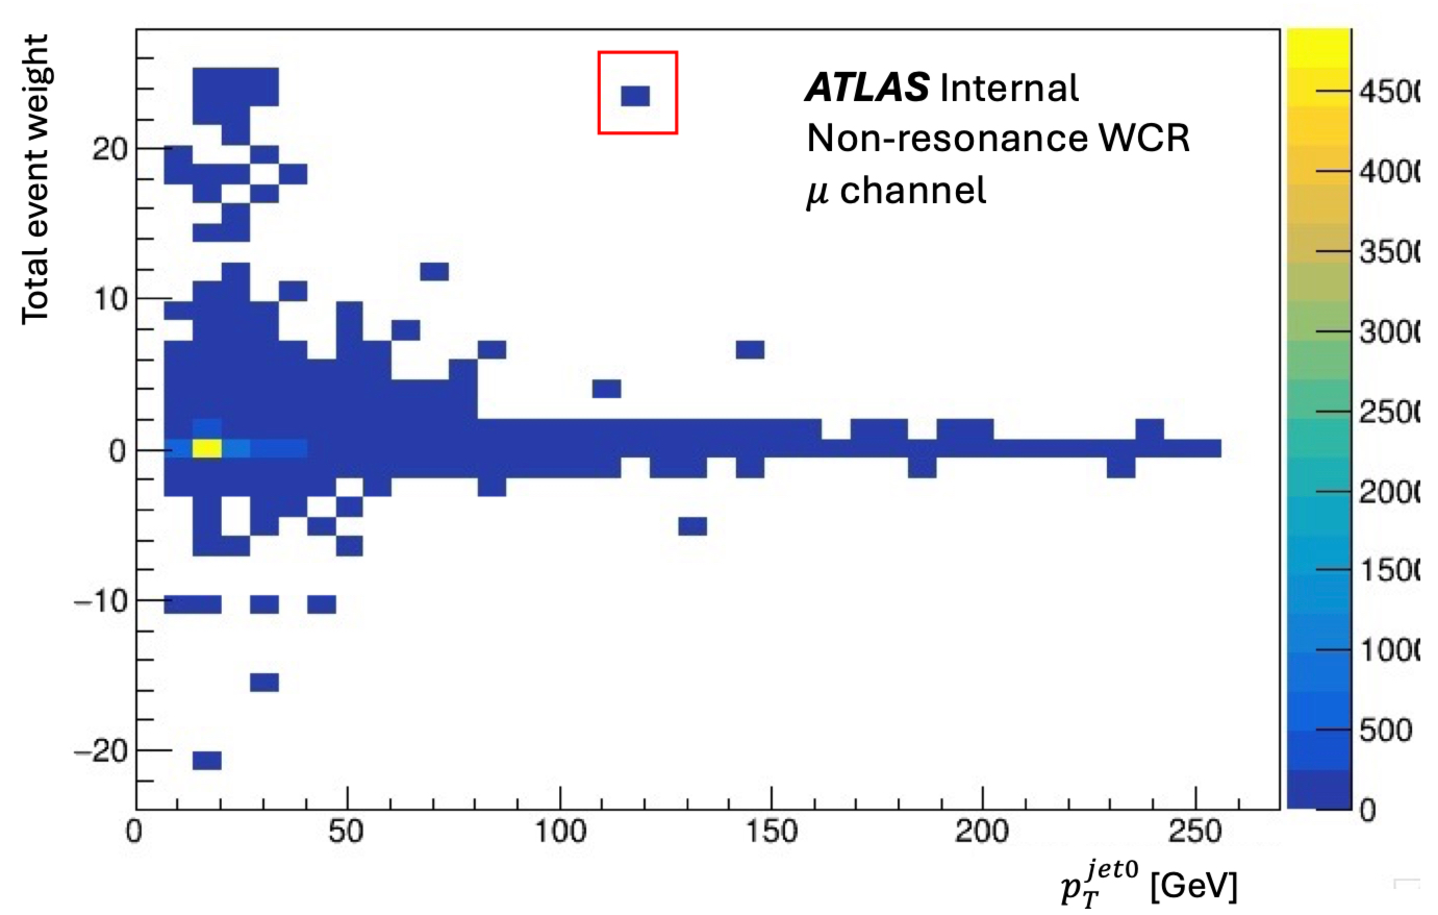
\includegraphics[width=\linewidth]{Figs/CH8/WCR_evenweight_mu.pdf}
        \caption[]{Event weights in the muon simulation}
    \end{subfigure}\par\medskip
    \caption[Electron--muon comparison in CRW-NonRes]{Electron--muon consistency checks in $\CRW$-$\NonRes$. In (a) and (b), red and blue denote the electron and muon channels, and the lower panels show their ratio. Panels (c) and (d) show the simulated event weights against leading-jet $\pT$. The marked high-weight muon event illustrates the statistical effect discussed in the text.}
    \label{fig:ch8_emu_comparison}
\end{figure}
